\chapter{AIDA-2020 testbeams}
\label{chapter:aidatestbeams}

\epigraph{I love fools' experiments. \\I am always making them.}{Charles Darwin}

One of the most important aspects of testing and developing \acrshort{DQM4hep} was to ensure that it was as generic as it was intended to be, and this meant deploying and using the framework on physics testbeams. \acrshort{DQM4hep} was originally developed during testbeams of the \acrfull{SiWECAL}, and its early testing phases were predominantly based on this detector, so it was apparent that it could be used in the originally-intended setting. However, in trying to develop it as a generic monitor, and to satisfy the requirements of a generic data monitoring and quality monitoring tool for AIDA-2020, it was essential that it was tested on other detectors of different types to demonstrate its generic nature. 

In this chapter, deployment, testing and usage of \acrshort{DQM4hep} on testbeams within the AIDA-2020 collaboration will be discussed in detail. For a testbeam where \acrshort{DQM4hep} was deployed outside of the AIDA-2020 community, see Chapter \ref{chapter:ideatestbeam}. Three testbeams will be described in detail, as they represent the different stages of using \acrshort{DQM4hep} as a data monitoring tool, from first implementation and deployment, to further developments, and finally as a mature tool integrated into the workflow of a testbeam.

\subsection*{CALICE testbeams}
The \acrshort{CALICE} testbeams were done with the \acrfull{FLC}\footnote{EN: Research with Lepton Colliders} group based at \acrshort{DESY} in Hamburg, working on the \acrfull{AHCAL} prototype during its development. Regular testbeams were held at the DESY II synchrotron at \acrshort{DESY} in Hamburg, Germany and at the \acrfull{SPS} at \acrshort{CERN} in Geneva, Switzerland. The goals for these testbeams varied over time but common focuses for the hardware were power-pulsing tests, and commissioning and calibration of new detector boards to test variations and changes to the manufacturing process. The testbeams were often used as testbeds for data acquisition electronics and software, such as the \acrshort{EUDAQ} data acquisition software, the \acrshort{BIF} device, and \acrshort{DQM4hep}.

\acrshort{DQM4hep} was used as an online monitoring and data quality monitoring tool for \acrshort{AHCAL} tesbeams beginning in May 2016, and in further testbeams between 2016 and 2018. The majority of these testbeams occurred at the DESY II facility, but two took place at the \acrshort{CERN} \acrshort{SPS} in May 2017 and June 2018.

\subsection*{The AHCAL prototype} % Full dossier on the AHCAL here: https://iopscience.iop.org/article/10.1088/1748-0221/5/05/P05004/pdf
The \acrfull{AHCAL} is a sampling calorimeter formed of steel absorber plates and plastic scintillator tiles, read out by silicon photomultipliers (\acrshort{SiPM}s) as active material\cite{proceedings-ahcal-prototype}. One of the important features of the \acrshort{AHCAL} is that the prototypes were designed to be made using techniques suitible for mass production, such as injection-moulding and automated foil-wrapping of the scintillator tiles, and pick-and-place assembly of the layers and their electronics. It also uses power pulsing -- rapidly cycling power so that the electronics are active only when the beam is present, according to a known beam structure. This helps to reduce power consumption and heat production, making cooling the layers easier.

\section{May 2016 at DESY II} % Wiki for this testbeam: http://flcwiki.desy.de/AHCALandBIF_TestBeamDESYMay2016
The first deployment of \acrshort{DQM4hep} on an \acrshort{AHCAL} testbeam was at DESY II during May 2016. The testbeam was to be two weeks in duration, following a one-week setup and preparation period. Besides testing the deployment and usage of DQM4hep, the goals of this testbeam where to test \acrshort{MIP} calibration of a new \acrshort{AHCAL} base unit (HBU), to test the power pulsing feature, and to perform \acrshort{TDC} calibrations. In addition to these goals for the \acrshort{AHCAL}, a device called a \acrfull{BIF}, another part of the ongoing work of AIDA-2020 Work Package 5, was being tested. 

Before and during the testbeam, the majority of the development for AHCAL-specific analysis modules was undertaken. Prior to this, \acrshort{DQM4hep} had only been used on \acrshort{SiWECAL} beams, and was untested for other detectors. 

File reader and streamer plugins for the \acrshort{LCIO} data format were already available in the now-deprecated \texttt{dqm4ilc} package, which meant that the framework could open and access the data format already.

\subsection{Data format}
The data for the \acrshort{AHCAL} is in the \acrfull{LCIO} format, using an object type called LCGenericObject, which is a generic format for use when the existing data formats are not suitable. It comprises two parts: the block of data itself, held in 14-bit numbers; and a header containing user-defined parameters, in this case a timestamp, a typename for the object, and a description of the data contained in the object.

The structure of a single event in LCGenericObject format can be seen below, which is the result of using the \texttt{dumpevent} tool to dump the contents of an \acrshort{LCIO} event to the command line:

\begin{verbatim}
--------------- print out of LCGenericObject collection --------------- 

  flag:  0x0
 parameter DAQquality [int]: 1, 
 parameter DataDescription [string]: i:CycleNr:i:BunchXID;i:EvtNr;i:
     ChipID;i:NChannels:i:TDC14bit[NC];i:ADC14bit[NC],
 parameter Timestamp [string]: Tue, 09 Feb 2016 18:20:43 +0100,
 parameter TypeName [string]: CaliceObject,

 [   id   ] i:Type,i:EventCnt,i:TS_Low,i:TS_High - isFixedSize: false
 --------------------------------------------------------
 [00000004]  i:0; i:15; i:15; i:0; i:36; i:12423; i:12422; i:12421;
     i:12420; i:12419; i:12418; i:12417; i:12416; i:12415; i:12414;
     i:12413; i:12412; i:12411; i:12410; i:12409; i:12408; i:12407;
     i:12406; i:12405; i:12404; i:12403; i:12402; i:12401; i:12400;
     i:12399; i:12398; i:12397; i:12396; i:12395; i:12394; i:12393;
     i:12392; i:12391; i:12390; i:12389; i:12388; i:12459; i:12458;
     i:12457; i:12456; i:12455; i:12454; i:12453; i:12452; i:12451;
     i:12450; i:12449; i:12448; i:12447; i:12446; i:12445; i:12444;
     i:12443; i:12442; i:12441; i:12440; i:12439; i:12438; i:12437;
     i:12436; i:12435; i:12434; i:12433; i:12432; i:12431; i:12430;
     i:12429; i:12428; i:12427; i:12426; i:12425; i:12424;
 --------------------------------------------------------
\end{verbatim}

% Thisis left here for convenience, but is from May 2017 at CERN
%\begin{verbatim}
%--------------- print out of LCGenericObject collection --------------- 
%
%  flag:  0x0
% parameter DAQquality [int]: 1, 
% parameter DataDescription [string]: i:CycleNr,i:BunchXID,i:EvtNr,
%     i:ChipID,i:NChannels,i:TDC14bit[NC],i:ADC14bit[NC], 
% parameter Timestamp [string]: Thu, 25 May 2017 05:38:25 +0200, 
% parameter TypeName [string]: CaliceObject, 
%
% [   id   ] i:Type,i:EventCnt,i:TS_Low,i:TS_High - isFixedSize: false
% --------------------------------------------------------
% [00000852] i:99; i:0; i:0; i:121; i:36; i:13365; i:13383; i:13378;
%     i:13370; i:13336; i:13351; i:13361; i:13365; i:13357; i:13338;
%     i:13345; i:13368; i:13386; i:13380; i:13386; i:13391; i:13382;
%     i:13363; i:13395; i:13342; i:13378; i:13335; i:13327; i:13376;
%     i:13342; i:13373; i:13406; i:13323; i:13361; i:13395; i:13378;
%     i:13365; i:13362; i:13378; i:13384; i:13355; i:12288; i:12288;
%     i:12288; i:12288; i:12288; i:12288; i:12288; i:12288; i:12288;
%     i:12288; i:12288; i:12288; i:12288; i:12288; i:12288; i:12288;
%     i:12288; i:12288; i:12288; i:12288; i:12288; i:12288; i:12288;
%     i:12288; i:12288; i:12288; i:12288; i:12288; i:12288; i:12288;
%     i:12288; i:12288; i:12288; i:12288; i:12288; i:12288;
% --------------------------------------------------------
%\end{verbatim}

In this case, the \texttt{TDC14bit[NC]} and \texttt{ADC14bit[NC]} are arrays, each holding a number of elements equal to the \texttt{NChannels} variable, in this case 36. Each element of these arrays corresponds to a single physical scintillator tile within the detector, and identifies which chip it belongs to using \texttt{ChipID}. 

The \texttt{ADC14bit} and \texttt{TDC14bit} arrays contain binary data, which is represented above converted directly to decimal. However some bits represent data other than the actual \acrshort{ADC} or \acrshort{TDC}, such as validation bits, hit bits, etc. An explanation of the structure of these bits can be seen in [ref].

[...] % Need to find the bit structure, maybe on a presentation Adrian gave?

\subsection{Results}
Over the course of the preparation week, the foundations were laid for the analysis module. This involved gaining a familiarity with the data structure, loading data from previous testbeams into \acrshort{DQM4hep} offline, and attempting to read it in basic ways. The first module was not ready for the beginning of the testbeam proper, but a few days afterwards we were able to produce plots in \acrshort{DQM4hep} from ``nearly-online'' testbeam data.

The first analysis module developed was the \texttt{AHCALRawModule}. The majority of the processing in this module was decoding of the data from the binary format and extracting the information from it. After this, validation bits and hit bits in the data were checked to classify data as `good' or `bad' hits. Then the actual \acrshort{ADC}s and \acrshort{TDC}s were filled into their respective histograms. 

The first module acted as a proof-of-concept, and once this was done further work started on creating more modules with a wider variety of features and plots to provide better coverage for online monitoring. We created and refined two separate modules during this testbeam -- \texttt{AHCALRawModuleChannel} and \texttt{AHCALRawModuleGlobal}. 

The channel module created a per-spectrum channel of all \acrshort{ADC}s, integrated over the whole run. It was able to load a number of individual channels, though due to the memory requirement, it could not track all channels simultaneously. To work around this, we implemented a facility for the module to read which channels to monitor from the \acrshort{XML} steering file, so that these could be defined at runtime. An example of some of the per-channel spectra created using this module can be seen in Fig. \ref{figure:aida/may2016/channelmodule}

\begin{figure}[p]
	\centering
	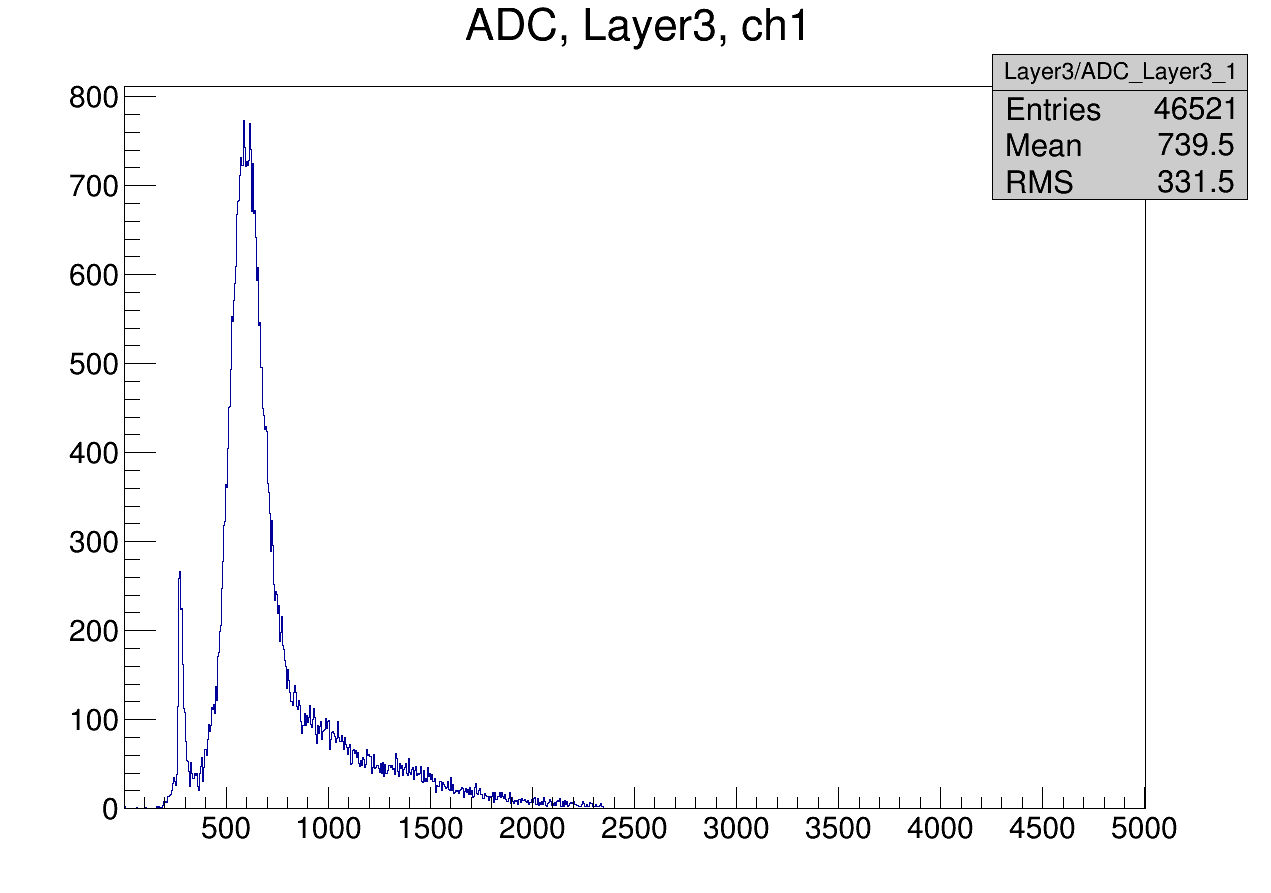
\includegraphics[width=0.95\textwidth]{../Pictures/ChannelModule-May2016.png} % Add an x-axis label to this too
	\caption{Histogram produced by \texttt{AHCALRawModuleChannel} showing an \acrshort{ADC} spectrum of a single channel for one run. The pedestal can be seen at approximately 300 and the \acrshort{MIP} peak at around 650.}
	\label{figure:aida/may2016/channelmodule}
\end{figure}

% We should use the ADC500 one here, because that makes sure that we remove the pedestal from the data and gives a better "signal" histogram
\begin{figure}[p]
	\centering
	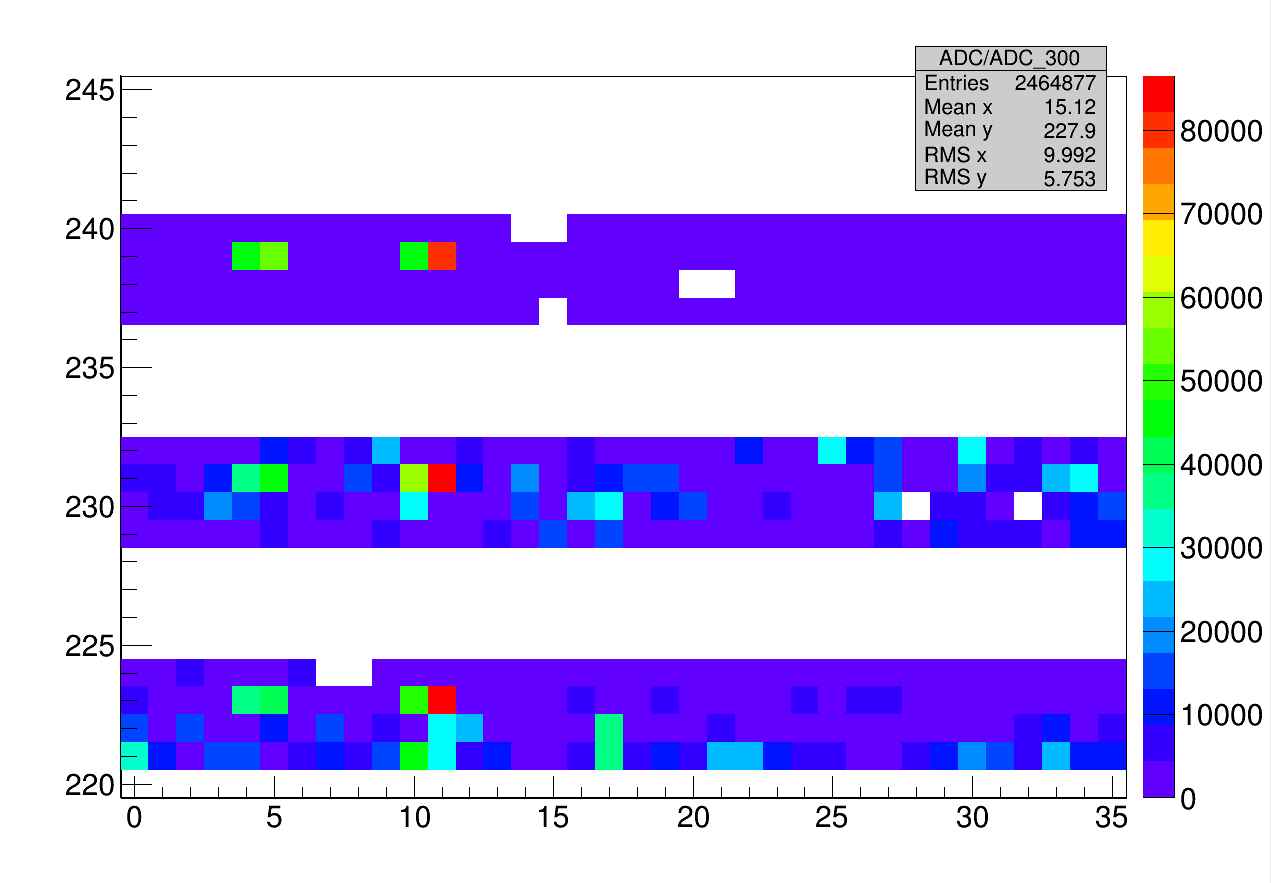
\includegraphics[width=0.85\textwidth]{../Pictures/GlobalModule-May2016.png} % Add axis labels: x is channel no., y is ChipID
	\caption{Histogram produced by \texttt{AHCALRawModuleGlobal} showing all \acrshort{ADC}s exceeding 300 over a single run. Dead or nonresponsive channels are seen as white squares. The horizontal gaps are due to the fact that some ChipIDs were not present.}
	\label{figure:aida/may2016/globalmodule}
\end{figure}

The global module produced a 2D histogram containing cells for each channel, coloured for the \acrshort{ADC} in that channel. This didn't produce a hitmap as the geometry information was not available in this plot, but did allow easy identification of dead channels and channels that were in the beamspot. An example of this can be seen in Fig. \ref{figure:aida/may2016/globalmodule}.

Overall, once the monitoring had been set up and initial bugs and problems fixed, it became a routine tool of the testbeam. This was made easier by the usage of \acrshort{XML} steering files for the monitoring interface canvases, allowing groups of plots and histograms to be automatically opened when the monitoring interface was started. This meant that with little effort, all information necessary for monitoring was easily available.

An example of the monitoring interface in use can be seen in Fig. \ref{figure:aida/may2016/overview}.

\begin{figure}[t]
	\centering
	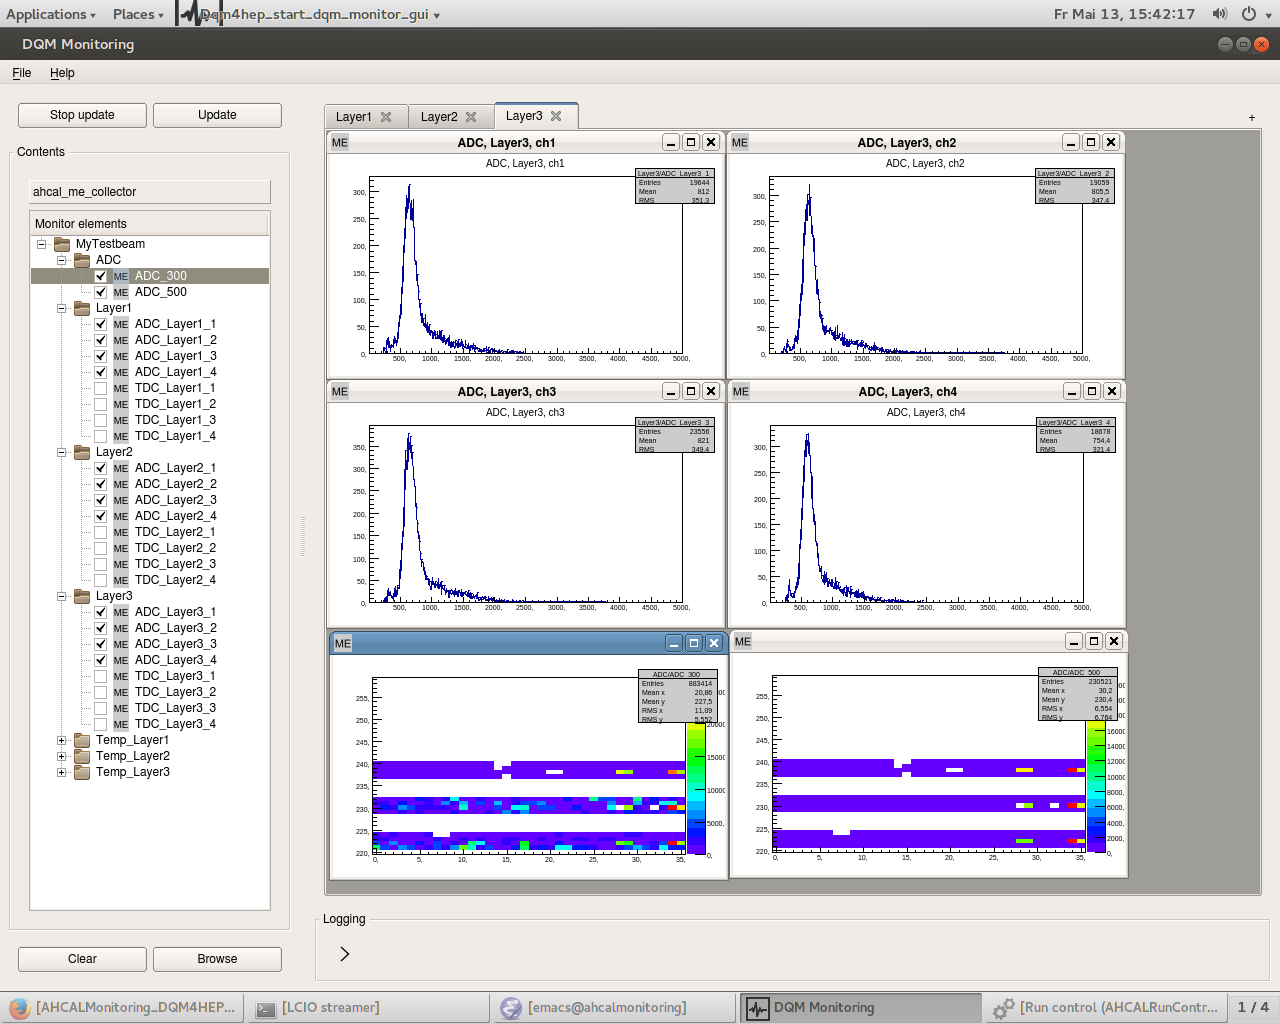
\includegraphics[width=0.95\textwidth]{../Pictures/PowerPulsingMipScans-May2016.png}
	\caption{A full screencapture from the May 2016 testbeam showing the monitoring interface in use during power pulsing tests, displaying a \acrshort{MIP} scan.}
	\label{figure:aida/may2016/overview}
\end{figure}

\section{July 2016 DESY II}
The next usage of \acrshort{DQM4hep} was a testbeam during July 2016, also at the DESY II facility. The testbeam was to be one week long, with a one-week preparation period. The primary goal for \acrshort{DQM4hep} in this testbeam was to establish hitmaps of the calorimeter. This would give a visual representation of the layers, allowing identification of the beamspot, allowing dead or mis-calibrated channels to be identified visually.

Creating a hitmap for the \acrshort{AHCAL} was nontrivial, as the information coming from the data acquisition device and stored in LCIO format did not encode location. Each channel was instead identified by its ``electronics number'' -- a combination of the ChipID of the board the channel was located on, and the number of the channel on that board.

Each layer was formed of four boards (each one with a ChipID), each of which contained sixteen layers. The orientation of the boards, which boards were in a layer, and the order of the layers in the stack were all changeable, so an additional requirement for the hitmap function was that it could take an external geometry file that could be changed or automatically generated. 

\acrshort{DQM4hep} has internal functions for parsing \acrshort{XML} data, so an \acrshort{XML} file was chosen as the format to store the geometry data. By making this an \acrshort{XML} file, it avoided hard-coding the geometry into the framework itself, allowing the geometry data to be changed at runtime. \acrshort{XML} also has the benefit of being human-readable. The AHCAL team already used an internal format for the geometry file for offline processing after testbeams, which was constructed and converted into different fromats via a  shell script, so this could be replicated for the \acrshort{DQM4hep} \acrshort{XML} file.

For analysis modules needing geometry, the \acrshort{XML} file was given as a required parameter for the steering file, which then built a C++ map of the correspondence between electronics number and $(i,j,k)$ co-ordinates of each channel in memory during initialisation. Then a function called \texttt{electronicsToIJK} was written that took the electronics number as the argument and returned the position of the channel in geometric co-ordinates. A further function was written, called \texttt{IJKToElectronics}, that performed the opposite operation, but this was not used. 

Using these new functions, another analysis module called \texttt{AHCALHitmap} was written that created a two dimensional histogram, with each bin representing a channel on the $x$ and $y$ axes for a single layer. This histogram was then filled with with the \acrshort{ADC}s of that channel for the whole event, producing a hitmap.

The analysis modules for creating hitmaps were prepared ahead of the testbeam, and used extensively. They were used to identify channels that were dead or nonresponsive, as well as to confirm already-known nonresponsive channels.

\begin{figure}[p]
	\centering
	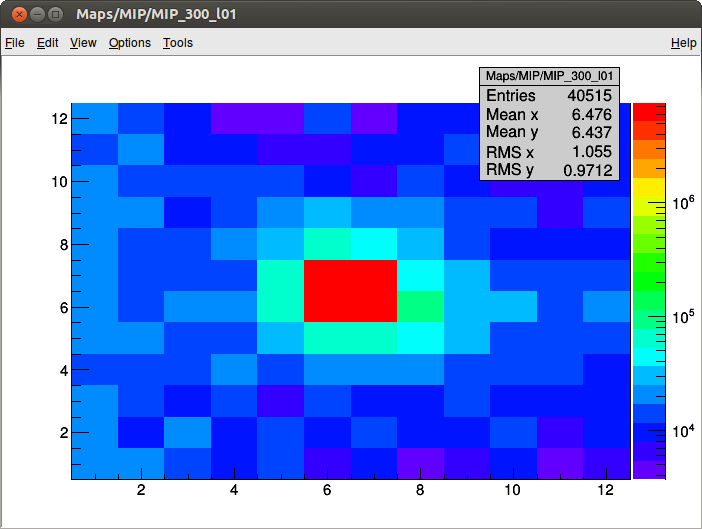
\includegraphics[width=0.95\textwidth]{../Pictures/AHCALHitmapSingle.png}
	\caption{A hitmap for a single layer during the July 2016 testbeam, showing all channels with \acrshort{ADC}s higher than 300. The beamspot is clearly visible in the centre.}
	\label{figure:aida/july2016/single-hitmap}
\end{figure}

\begin{figure}[p]
	\centering
	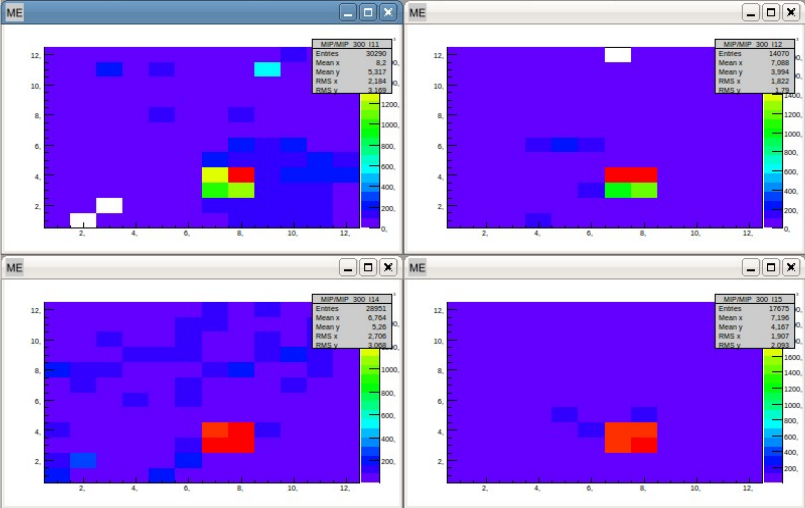
\includegraphics[width=0.95\textwidth]{../Pictures/AHCALHitmapFour.png}
	\caption{A collection of hitmaps for four layers in the stack during the July 2016 testbeam. The beamspot is visible, as are several dead or unresponsive channels in the top-left and top-right hitmaps.}
	\label{figure:aida/july2016/four-hitmap}
\end{figure}


\section{May 2017 at CERN SPS} % Wiki pages are here (http://flcwiki.desy.de/AHCALTestBeamCERN2017) but we ideally want an actual report for this.
During May 2017, testbeam time at the \acrshort{CERN} \acrfull{SPS} facility was used for further tests for the \acrshort{AHCAL}. One of the goals for this testbeam was to evaluate the performance of the power pulsing feature in magnetic fields up to 1.5T. The process of manufacturing the detector layers and boards was being automated, and a larger number of layers were available for this testbeam, so it also presented a way to test using a larger number of channels than before. 

Part of the programme for the testbeam was to use the electron and muon beams available at the \acrshort{SPS} for calibrating the newly-produced layers, as well as doing an energy scan with a pion beam.

The monitoring with \acrshort{DQM4hep} in this testbeam included analysis modules that monitored the individual channels of all 40 large layers, as well as producing hitmaps of several types, such as unweghted, \acrshort{ADC}-weighted, and near-pedestal. Standalone modules monitoring the temperature of the detector hardware was also used. 

At this point in the testbeam process, the online monitoring system with \acrshort{DQM4hep} had matured, partially due to the data format of the detector having been fixed for some time. Experience with running, using, and modifying the analysis modules had been disseminated throughout the team, and team members wrote their own analysis modules for producing plots.

Because of this, during the testbeam \acrshort{DQM4hep} was used as intended -- as a tool for shifters to use to diagnose and troubleshoot problems with the beams or detectors. A specific expert on \acrshort{DQM4hep} was not necessary, as enough people operating the testbeam understood \acrshort{DQM4hep} to be able to modify analysis modules on the fly according to their needs.

% In previous testbeams, analysis modules that produced correlation plots were developed by other team members,

%\begin{center}
%	[Photographs from the installation and testbeam area go here]
%\end{center}
%
%\begin{center}
%	[Plots from the testbeam]
%\end{center}

\begin{figure}[p]
	\centering
	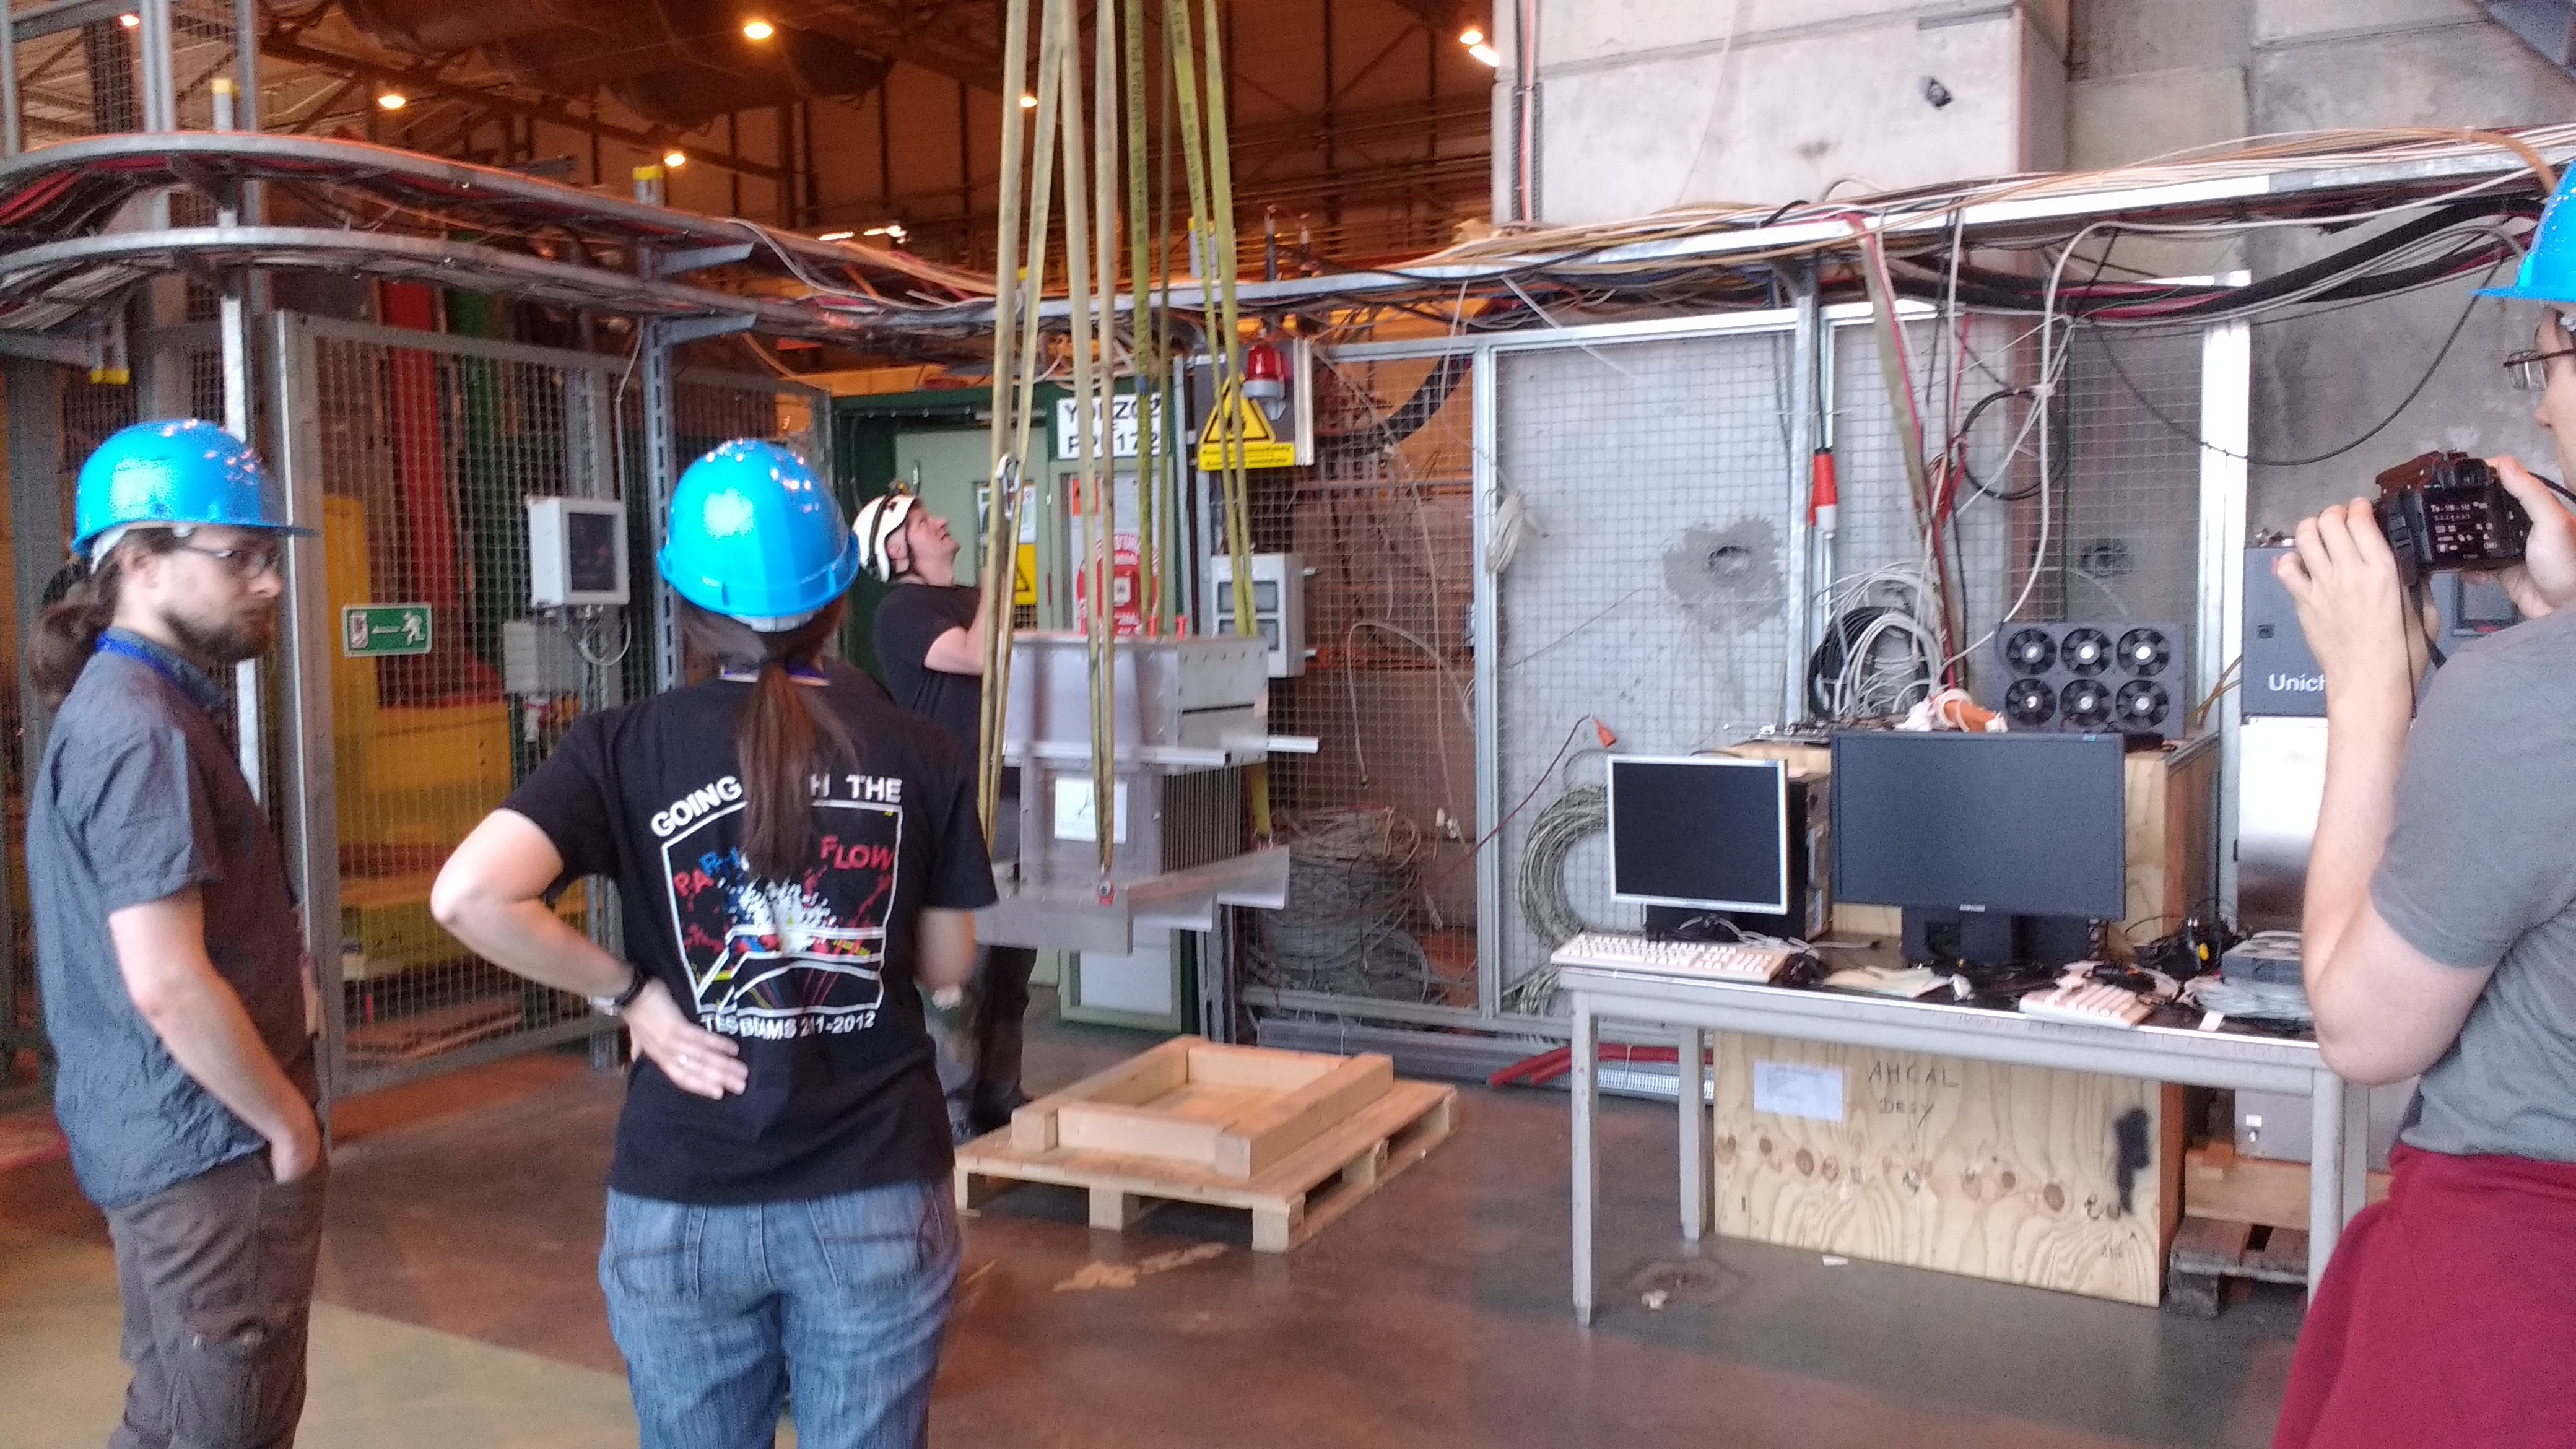
\includegraphics[width=0.85\textwidth]{../Pictures/AHCAL-CERN-2017-Installation-1.jpg}
	\caption{Installation 1}
	\label{figure:aida/may2017/installation-1}
\end{figure}

\begin{figure}[p]
	\centering
	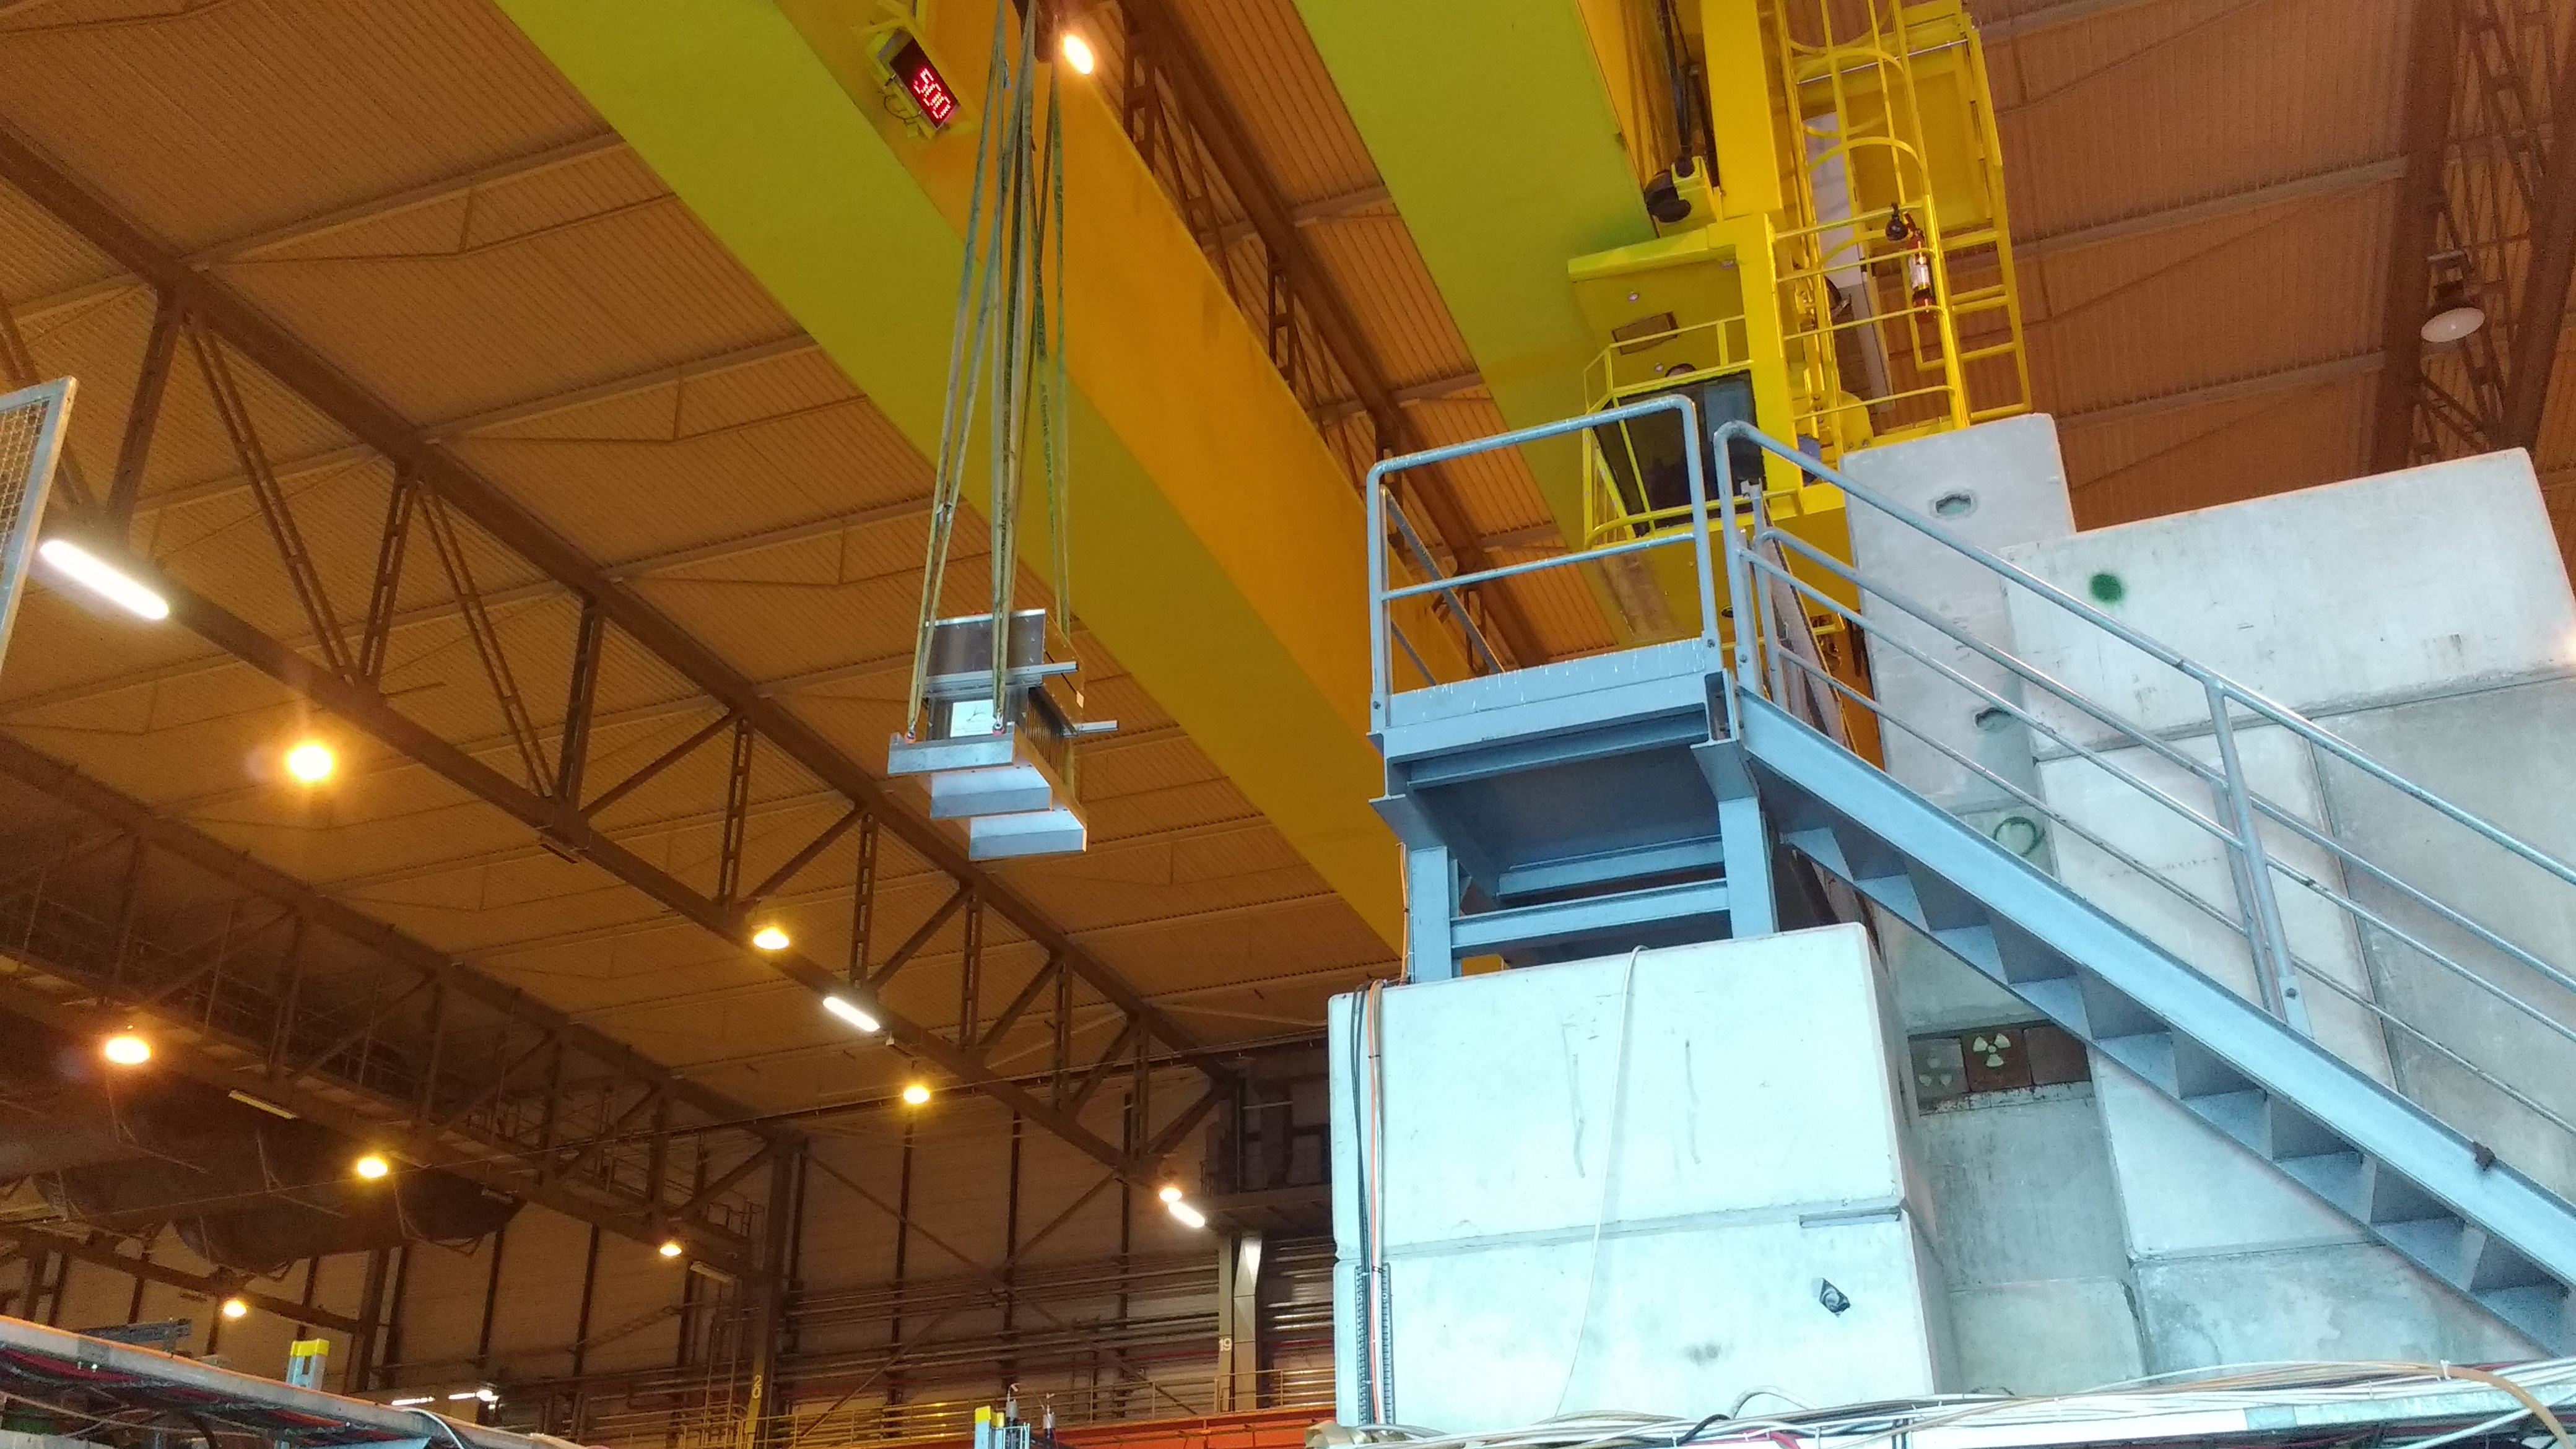
\includegraphics[width=0.85\textwidth]{../Pictures/AHCAL-CERN-2017-Installation-2.jpg}
	\caption{Installation 2}
	\label{figure:aida/may2017/installation-2}
\end{figure}

\begin{figure}[p]
	\centering
	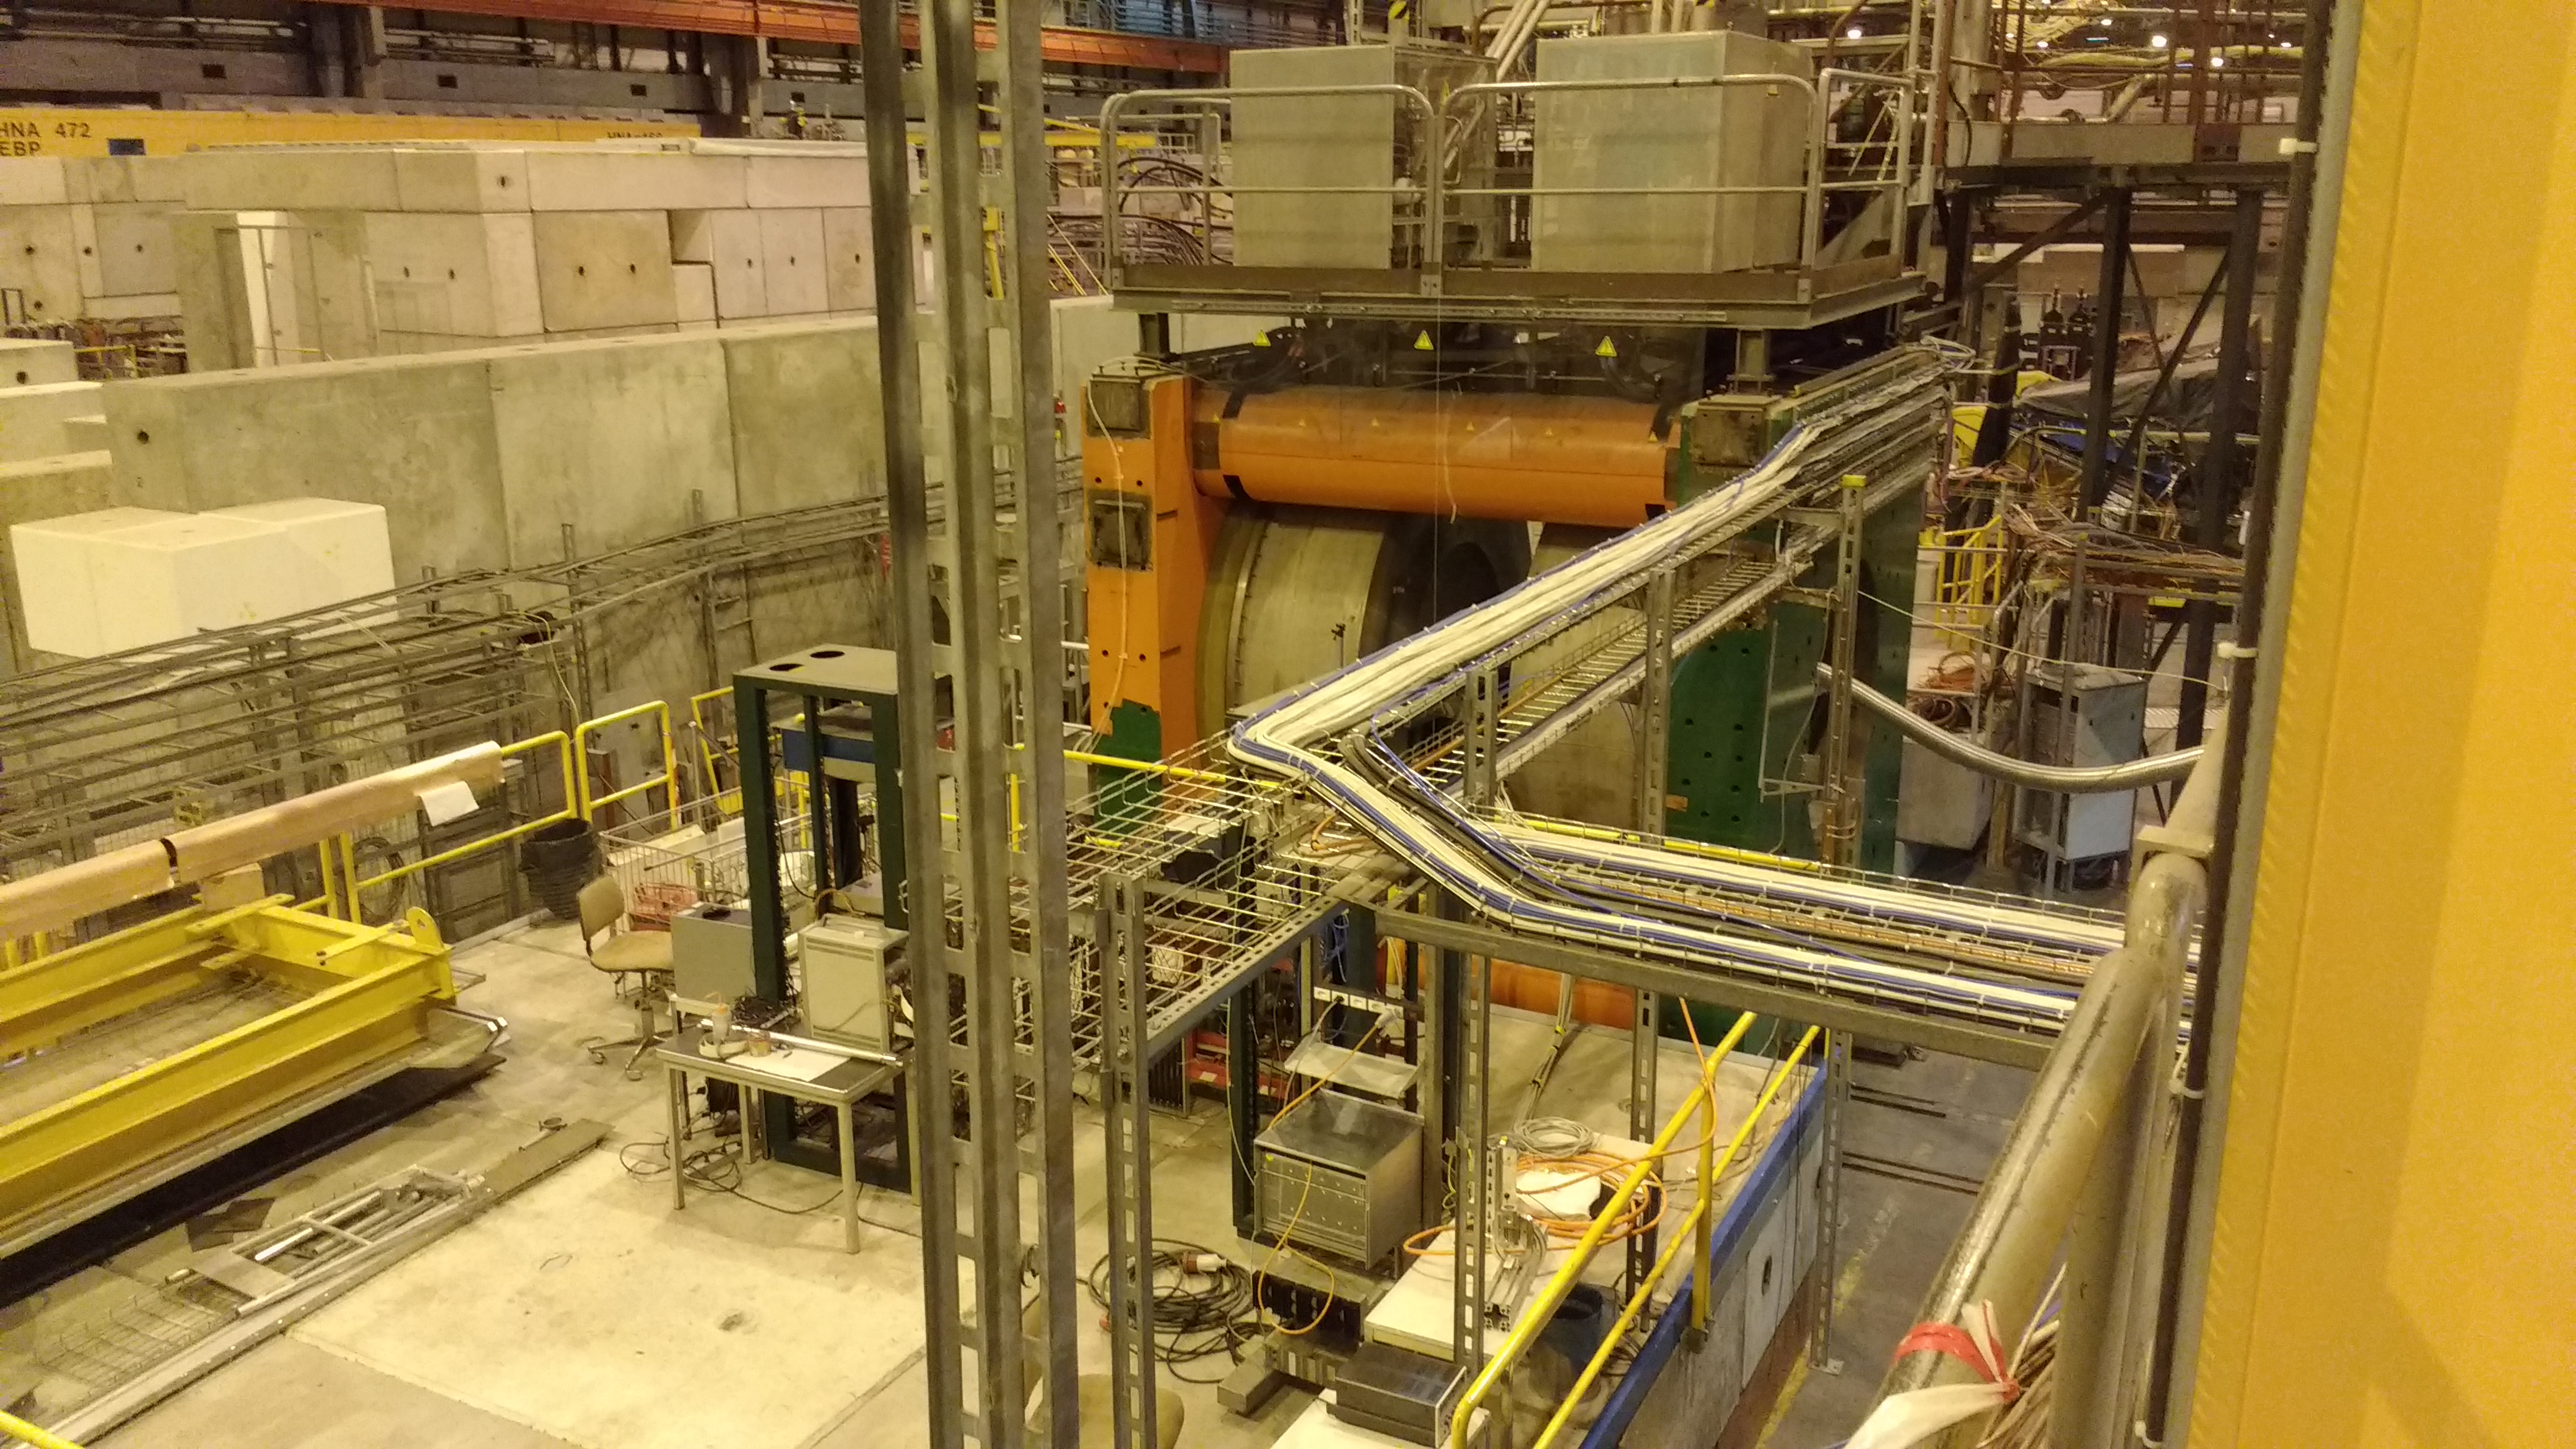
\includegraphics[width=0.85\textwidth]{../Pictures/AHCAL-CERN-2017-Area-1.jpg}
	\caption{Testbeam area 1}
	\label{figure:aida/may2017/area-1}
\end{figure}

\begin{figure}[p]
	\centering
	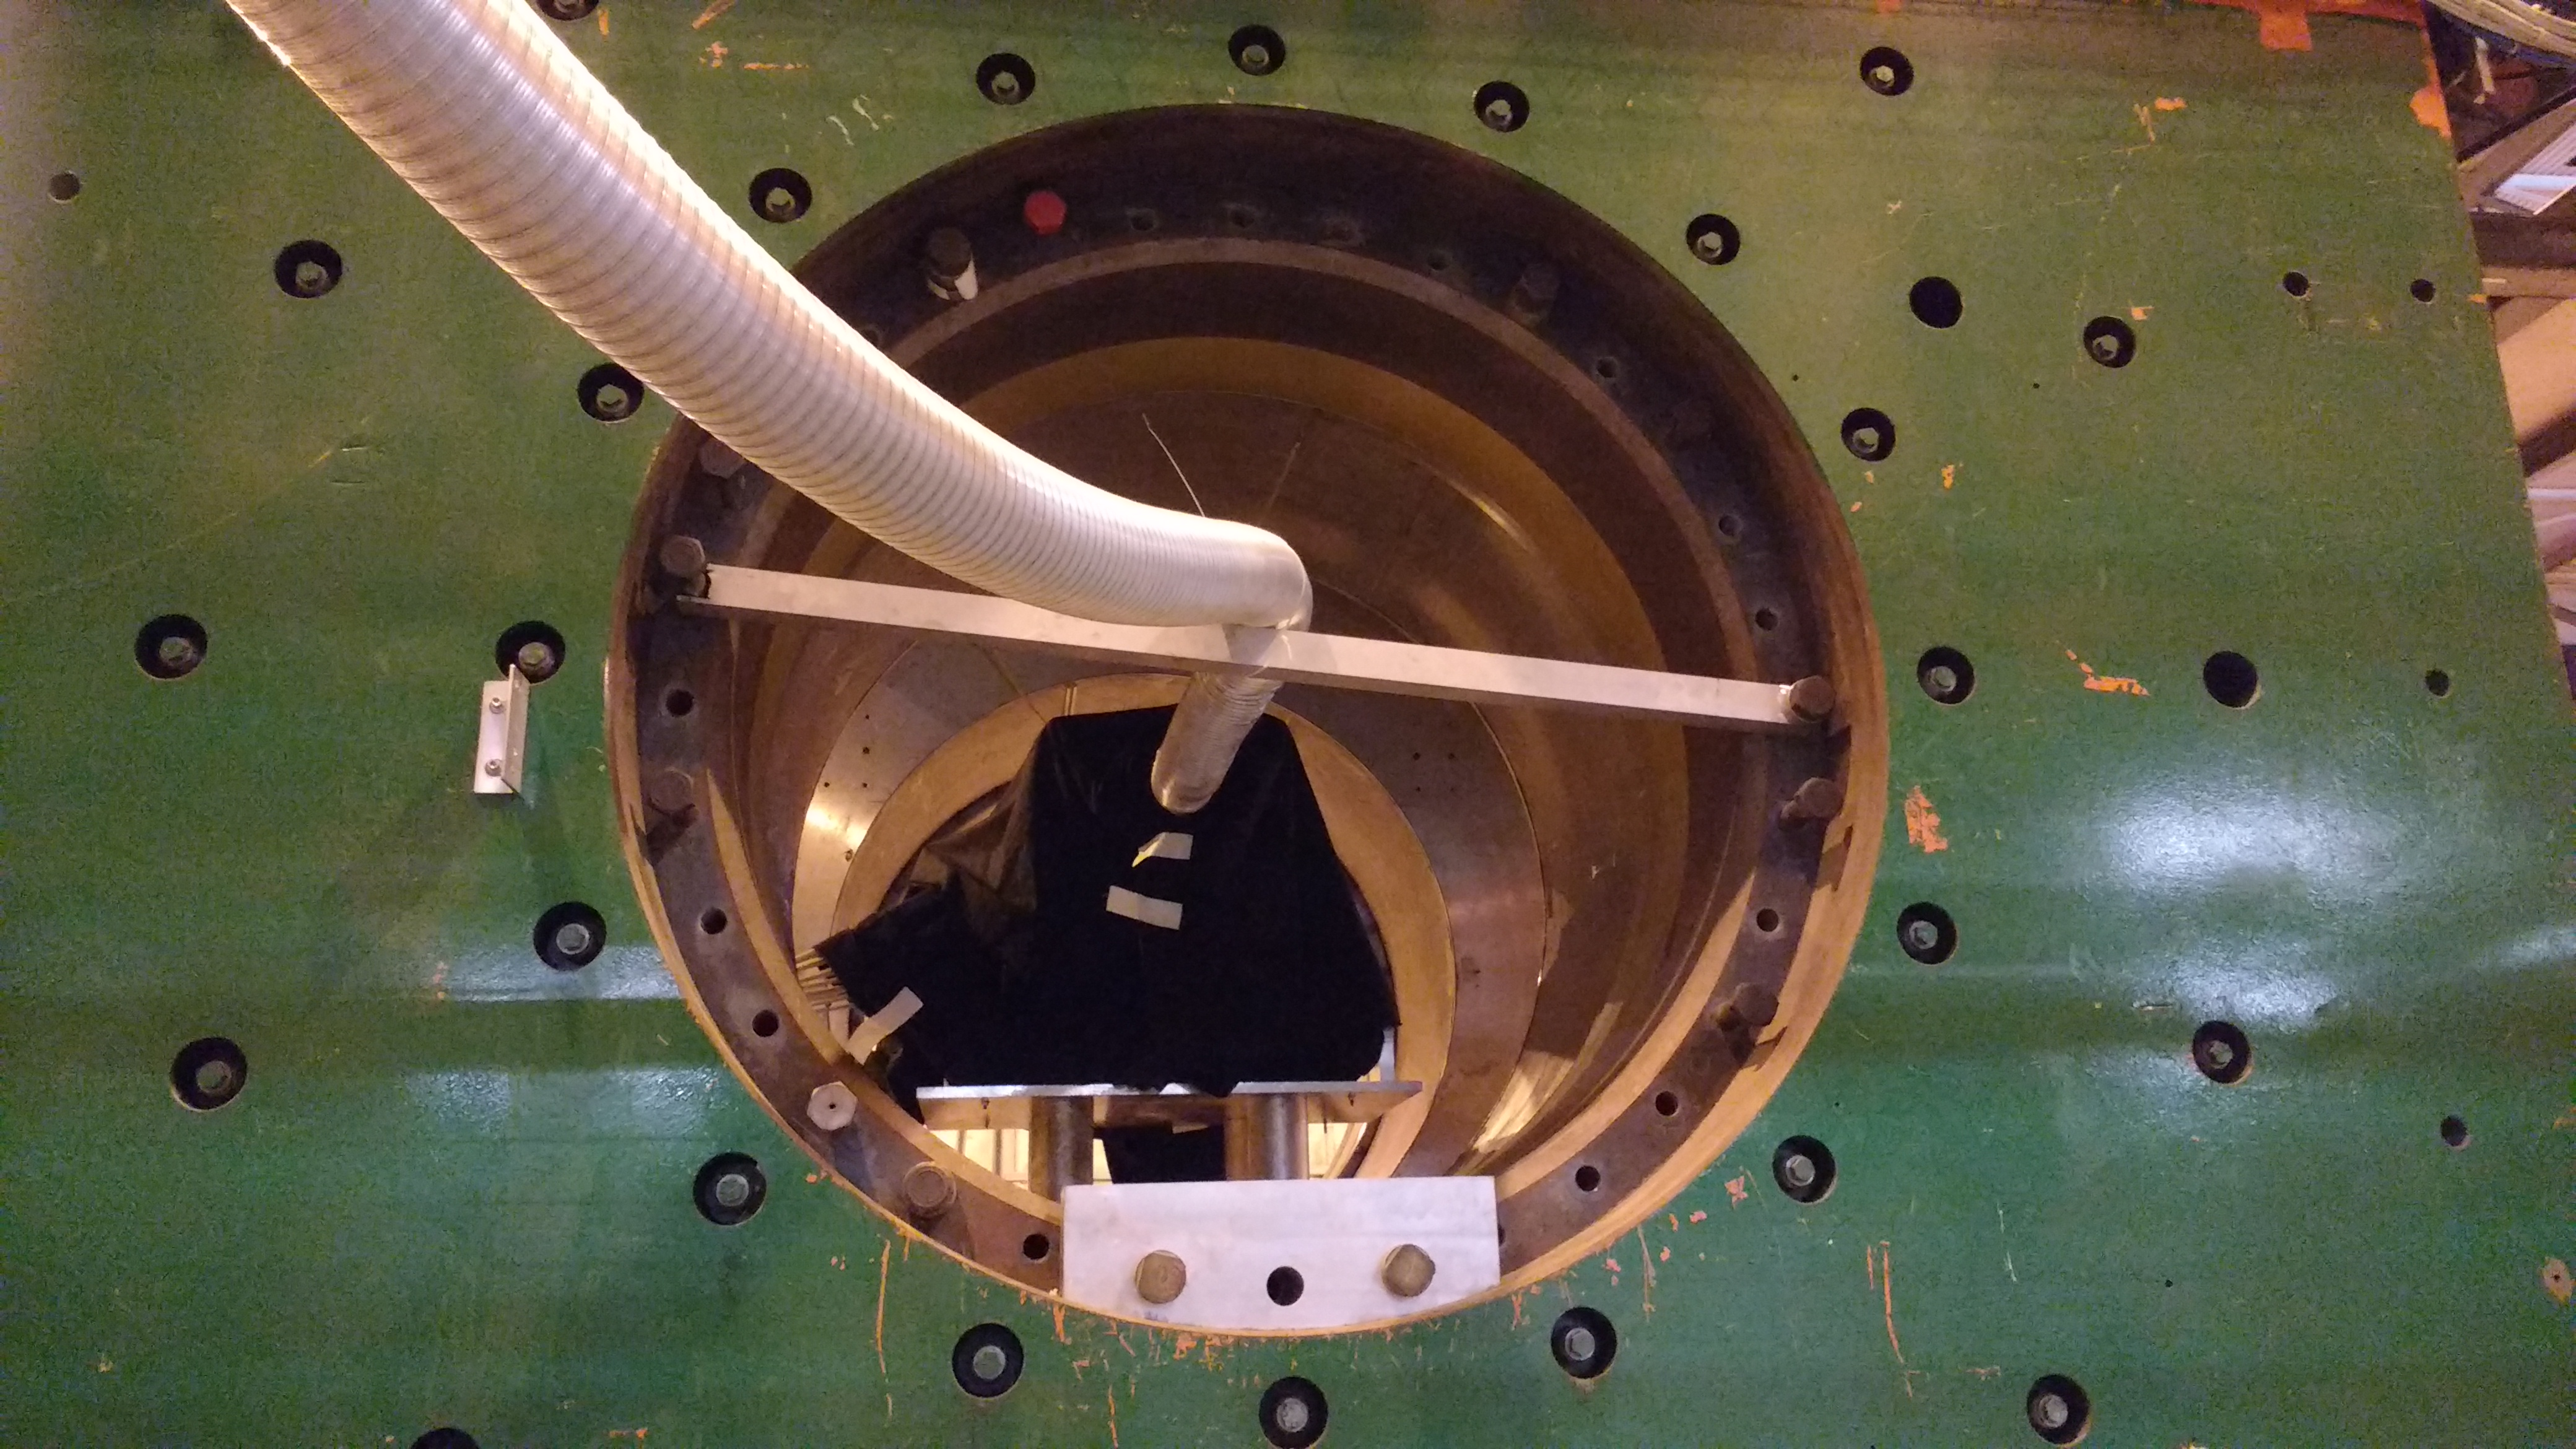
\includegraphics[width=0.85\textwidth]{../Pictures/AHCAL-CERN-2017-Area-2.jpg}
	\caption{Testbeam area 2}
	\label{figure:aida/may2017/area-2}
\end{figure}
